% !TEX root = IBL-InsolvabilityOfQuintic.tex
\chapter{Galois theory}
\label{chapter:GaloisTheory}
\thispagestyle{empty}

We finished Chapter~\ref{chapter:AlgebraicExtensions} by computing automorphism groups of field extensions. We also began to connect the subfields of an extension  field $L$ of $F$ to subgroups of $\Aut(L/F)$.  We  now narrow our focus on which types of extension fields we consider, and in doing so, we significantly sharpen what we can say about this connection. It will be lynchpin of our argument showing that not all polynomials over $\mathbb{Q}$ are solvable by radicals over $\mathbb{Q}$.

Also, from here on, we will exclusively focus on subfields of $\mathbb{C}$. This will streamline (and simplify) our work, but it will also slightly obscure the general theory. Which is to say, this is more the beginning of the story than the end. 

% % % % % % % % % % % % % % % % % % % % % % % % % % % % % % % % % % % % % % % % % % % %
% % % % % % % % % % % % % % % % % % % % % % % % % % % % % % % % % % % % % % % % % % % %
% SECTION
% % % % % % % % % % % % % % % % % % % % % % % % % % % % % % % % % % % % % % % % % % % %
% % % % % % % % % % % % % % % % % % % % % % % % % % % % % % % % % % % % % % % % % % % %
\section{Galois extensions and Galois groups}

\begin{definition}\label{def.SplittingField}
Let $F$ be a subfield of $\mathbb{C}$, and let $p(x) \in F[x]$. Define $F^{p(x)}$ to be the subfield of $\mathbb{C}$ generated by $F$ and all roots of $p(x)$; thus,  $F^{p(x)}=F(r_1,\ldots,r_n)$ where $r_1,\ldots,r_n$ are all of the roots of $p(x)$ in $\mathbb{C}$.
\end{definition}

For example, if  $p(x) = x^5 - 1$, then by Theorem~\ref{thm.nthRoots1}, the roots of $p(x)$ are $1,\zeta_5,\zeta_5^2,\zeta_5^3,\zeta_5^4$, so $\mathbb{Q}^{p(x)}=\mathbb{Q}(1,\zeta_5,\zeta_5^2,\zeta_5^3,\zeta_5^4)$.

\begin{problem}\label{prob.QAdjoinZeta5IsGalois}
Let $p(x) = x^5 - 1$. Use Theorem~\ref{thm.FieldAdjoinElementsContainedInField} to explain why $\mathbb{Q}^{p(x)}=\mathbb{Q}(\zeta_5)$.
\end{problem}

\begin{problem}\label{prob.QAdjoinCubeRoot2IsNotASplittingField}
Let $p(x) = x^3 - 2$. Explain why $\mathbb{Q}^{p(x)}\neq\mathbb{Q}(\sqrt[3]{2})$.
\end{problem}

\begin{problem}\label{prob.ShowFieldIsASplittingField}
For each field $F$ below, find a polynomial $p(x)\in \mathbb{Q}[x]$ such that $F=\mathbb{Q}^{p(x)}$.
\begin{multicols}{2}
\begin{enumerate}
\item $F=\mathbb{Q}(\sqrt{2})$
\item $F=\mathbb{Q}(\sqrt{2},i)$
\item $F=\mathbb{Q}(\sqrt[3]{2},\zeta_3)$
\item $F=\mathbb{Q}(\zeta_{12})$
\end{enumerate}
\end{multicols}
\end{problem}

\begin{definition}
Let $F\subseteq K$ be subfields of $\mathbb{C}$.
\begin{enumerate}
\item We say that $K$ is a \textbf{Galois extension} of $F$ if $K = F^{p(x)}$ for some $p(x) \in F[x]$.
\item If $K$ is a Galois extension of $F$, then $\Aut(K/F)$ is called the \textbf{Galois group} of $K$ over $F$.
\end{enumerate}
\end{definition}

Revisiting Problem~\ref{prob.ShowFieldIsASplittingField} with this new terminology, we see that each of $\mathbb{Q}(\sqrt{2})$, $\mathbb{Q}(\sqrt{2},i)$, $\mathbb{Q}(\sqrt[3]{2},\zeta_3)$, and $\mathbb{Q}(\zeta_{12})$ are Galois extensions of $\mathbb{Q}$. Also, Problem~\ref{prob.QAdjoinCubeRoot2IsNotASplittingField} hints at the fact that $\mathbb{Q}(\sqrt[3]{2})$ might not be a Galois extension of $\mathbb{Q}$ (but there is more to prove to establish that).

Let's generalize parts of Problem~\ref{prob.ShowFieldIsASplittingField} and record some types of extensions that are always Galois.

\begin{theorem}\label{thm.QAdjoinSquareRootIsGalois}
Let $a\in \mathbb{Q}$. Then $\mathbb{Q}(\sqrt{a})$ is a Galois extension of $\mathbb{Q}$.
\end{theorem}

\begin{theorem}\label{thm.QAdjoinZetanIsGalois}
Let $n$ be a positive integer. Then $\mathbb{Q}(\zeta_{n})$ is a Galois extension of $\mathbb{Q}$.
\end{theorem}

As mentioned above, $\mathbb{Q}(\sqrt[3]{2})$ might not be a Galois extension of $\mathbb{Q}$, but it is true that  $F(\sqrt[3]{2})$ a Galois extension of $F$ provided $F$ contains $\zeta_3$. The next theorem addresses this.

\begin{theorem}\label{thm.QAdjoinRadicalIsGaloisOverFieldWithRootsUnity}
Let $F$ be a subfield of $\mathbb{C}$. Suppose that $r\in \mathbb{C}$ and $r^n\in F$ for some positive integer $n$. If $\zeta_n\in F$, then $F(r)$ is a Galois extension of $F$.
\end{theorem}

% % % % % % % % % % % % % % % % % % % % % % % % % % % % % % % % % % % % % % % % % % % %
% SUBSECTION
% % % % % % % % % % % % % % % % % % % % % % % % % % % % % % % % % % % % % % % % % % % %
\subsection{Size of Galois groups}
The next fact highlights the importance of Galois extensions. The point is roughly that the automorphism group of a Galois extension has the ``expected'' number of automorphisms; whereas, automorphism groups of non-Galois extension will necessarily have fewer.

\begin{fact}\label{fact.SizeGaloisGroup}
Let $F\subseteq K$ be subfields of $\mathbb{C}$. If $K$ is a Galois extension of $F$,  $|\Aut(K/F)| = [K:F]$.
\end{fact}

Fact~\ref{fact.SizeGaloisGroup} is extremely powerful. Let's start by seeing how it can help streamline the computation of certain automorphism groups.

\begin{problem}\label{prob.AutQAdjoinCubeRoot2AndZeta3OverQ}
Let $L = \mathbb{Q}(\sqrt[3]{2},\zeta_3)$. Let's determine $\Aut(L/\mathbb{Q})$. Recall from Problem~\ref{prob.ShowFieldIsASplittingField} that $L$ is a Galois extension of $\mathbb{Q}$.  
\begin{enumerate}
\item What is minimal polynomial for $\sqrt[3]{2}$ over $\mathbb{Q}$? Why?
\item What is minimal polynomial for $\zeta_3$ over $\mathbb{Q}(\sqrt[3]{2})$? Why?
\item Use Fact~\ref{fact.BasisChainExtensionField} to explain why $[L : \mathbb{Q}] = 6$.
\item Let $\phi\in  \Aut(\mathbb{Q}(\sqrt[3]{2},\zeta_3)/\mathbb{Q})$. Use Theorem~\ref{thm.HomFixingFPermutesRootsOfPolysOverF} to explain why there are only 3 choices for $\phi(\sqrt[3]{2})$ and only two choices for $\zeta_3$. What are they?
\item Complete the table of possible elements of $\Aut(L/\mathbb{Q})$.
\begin{center}
\tabulinesep = 2mm
\begin{tabu} {X[$r,m]|[2pt]X[$c,m]|X[$c,m]|X[$c,m]|X[$c,m]|X[$c,m]|X[$c,m]}
 & \phi_1 & \phi_2 & \phi_3 & \phi_4  & \phi_5 & \phi_6\\ \tabucline[2pt]{-}
\sqrt[3]{2} \; \mapsto\;  & \sqrt[3]{2} &  &  & & &\\  \hline
\zeta_3 \; \mapsto \; & \zeta_3 &  &  &  & & 
\end{tabu}
\end{center}
\item Use Fact~\ref{fact.SizeGaloisGroup} to explain why every function in the table above must be in $\Aut(L/\mathbb{Q})$.
\end{enumerate}
\end{problem}

\begin{problem}\label{prob.AutQAdjoinCubeRoot2AndZeta3OverQLattices}
Let's revisit $L = \mathbb{Q}(\sqrt[3]{2},\zeta_3)$ from Problem~\ref{prob.AutQAdjoinCubeRoot2AndZeta3OverQ} and connect subfields of $L$ with subgroups of $\Aut(L/\mathbb{Q})$ using Theorem~\ref{thm.AutLOverKSubgroupAutLOverF}. The following are subfields of $L$.
\[K_0 = \mathbb{Q}(\zeta_3)\quad K_1 = \mathbb{Q}(\sqrt[3]{2})\quad K_2 = \mathbb{Q}(\sqrt[3]{2}\zeta_3)\quad \quad K_3 = \mathbb{Q}(\sqrt[3]{2}\zeta_3^2)\]
\begin{enumerate}
\item Compute $\Aut(L/K_0)$, $\Aut(L/K_1)$, $\Aut(L/K_2)$, and $\Aut(L/K_3)$ by determining which of  $\phi_1,\ldots,\phi_6$ are in each one.
\item Use Theorem~\ref{thm.AutLOverKSubgroupAutLOverF} to organize your findings by writing the appropriate elements in the boxes in the subgroup lattice of $\Aut(L/\mathbb{Q})$. 
\begin{itemize}
\item Label the degree of each field extension on the lines of the lattice on the left. Fact~\ref{fact.BasisChainExtensionField} should help. A couple have been done for you.
\item Label the order and index of each subgroup on the lines of the lattice on the right.   
\end{itemize} 
\end{enumerate}
\begin{center}
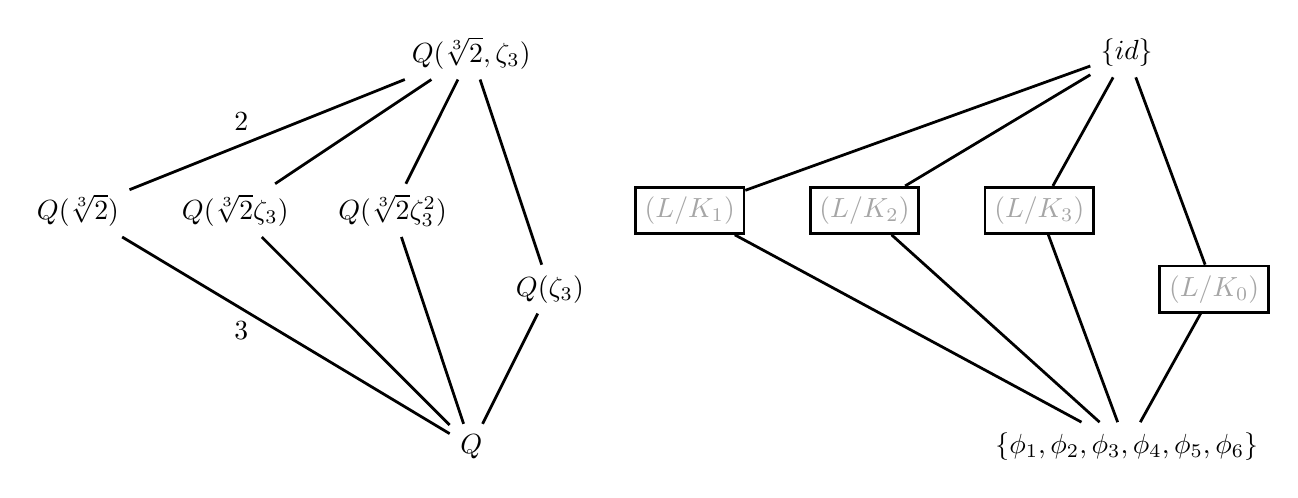
\begin{tikzpicture}[line width = 1, xscale = 1.11]
\begin{scope}[xscale = 0.9]
\node (L) at (0,4) {$\mathbb{Q}(\sqrt[3]{2},\zeta_3)$}; 
\node (K1) at (-5,2) {$\mathbb{Q}(\sqrt[3]{2})$}; 
\node (K2) at (-3,2) {$\mathbb{Q}(\sqrt[3]{2}\zeta_3)$}; 
\node (K3) at (-1,2) {$\mathbb{Q}(\sqrt[3]{2}\zeta_3^2)$}; 
\node (K0) at (1,1) {$\mathbb{Q}(\zeta_3)$}; 
\node (F) at (0,-1) {$\mathbb{Q}$};

\foreach \i in {0,1,2,3} {\draw (F) -- (K\i);}
\foreach \i in {0,1,2,3} {\draw (L) -- (K\i);}

\node[anchor = 45] at (-2.7,0.7) {$3$};
\node[anchor = -45] at (-2.7,2.9) {$2$};

%\draw[line width = 0.8, ->] (1.5,4) -- (5.5,4);
%\draw[line width = 0.8, ->] (3,2) -- (4,2);
%\draw[line width = 0.8, ->] (1.5,0) -- (5.5,0);
\end{scope}

\begin{scope}[shift = {(7.5,0)}]
\node (L) at (0,4) {$\{\text{id}\}$}; 
\node[draw] (K1) at (-5,2) {\textcolor{black!35}{$\Aut(L/K_1)$}}; 
\node[draw] (K2) at (-3,2) {\textcolor{black!35}{$\Aut(L/K_2)$}};
\node[draw] (K3) at (-1,2) {\textcolor{black!35}{$\Aut(L/K_3)$}};
\node[draw] (K0) at (1,1) {\textcolor{black!35}{$\Aut(L/K_0)$}}; 
\node (F) at (0,-1) {$\{\phi_1, \phi_2,\phi_3,\phi_4,\phi_5,\phi_6\}$};

\foreach \i in {0,1,2,3} {\draw (F) -- (K\i);}
\foreach \i in {0,1,2,3} {\draw (L) -- (K\i);}
\end{scope}

\end{tikzpicture}
\end{center}
\begin{enumerate}[resume]
\item What familiar group is $\Aut(L/\mathbb{Q})$ isomorphic to?
\end{enumerate}
\end{problem}

\begin{problem}\label{prob.QAdjoinCubeRoot2OverQNotGalois}
Use Fact~\ref{fact.SizeGaloisGroup} and Problem~\ref{prob.AutQAdjoinCubeRoot2OverQ} to argue that  $\mathbb{Q}(\sqrt[3]{2})$ is \emph{not} a Galois extension of $\mathbb{Q}$ 
\end{problem}

% % % % % % % % % % % % % % % % % % % % % % % % % % % % % % % % % % % % % % % % % % % %
% SUBSECTION
% % % % % % % % % % % % % % % % % % % % % % % % % % % % % % % % % % % % % % % % % % % %
\subsection{Galois groups as permutation groups}
We now explore how to look at Galois groups as groups of permutations. The key, yet again, is Theorem~\ref{thm.HomFixingFPermutesRootsOfPolysOverF}. We begin by recalling a some definitions from group theory.

\begin{definition}
Let $X$ be a set. A bijection from $X$ to $X$ is called a \textbf{permutation} of $X$. The set of all permutations of $X$ is denoted $\operatorname{Sym}(X)$. 
The set of all permutations of $\{1,\ldots,n\}$ is usually denoted by $S_n$ (instead of $\operatorname{Sym}(\{1,\ldots,n\})$.
\end{definition}

Recall that, for any set $X$, $\operatorname{Sym}(X)$ is a group with respect to function composition. The identity is the identity function, denoted id.

\begin{theorem}\label{thm.GaloisGroupIsPermGroup}
Let $F$ be a subfield of $\mathbb{C}$. Let $p(x)\in F(x)$, and let $R$ be the set of all of roots of $p(x)$ in $\mathbb{C}$.  
\begin{enumerate} 
\item If $\phi \in \Aut(F^{p(x)}/F)$, then $\phi(R) = R$. Thus, if $\phi^R: R\rightarrow R$ is the restriction of $\phi$ to $R$, then  $\phi^R\in \operatorname{Sym}(R)$.
\item The map $f: \Aut(F^{p(x)}/F)\to \operatorname{Sym}(R)$ where $f(\phi)=\phi^R$  is an injective homomorphism. 
\end{enumerate}
Consequently, $\Aut(F^{p(x)}/F)$ is isomorphic to a subgroup of $\operatorname{Sym}(R)$.
\end{theorem}

\begin{corollary}\label{cor.GaloisGroupIsPermGroup}
Let $F$ be a subfield of $\mathbb{C}$. Let $p(x)\in F(x)$ be a polynomial of degree $n$. Then $\Aut(F^{p(x)}/F)$ is isomorphic to a subgroup of $S_n$.
\end{corollary}

To view $\Aut(F^{p(x)}/F)$ as a subgroup of $S_n$, we just need to label the roots of $p(x)$ by $1,\ldots,n$ in some way and then record how each element of $\Aut(F^{p(x)}/F)$ permutes the roots. Let's take a look at an example of this.

\begin{example}\label{exam.QAdjoinZeta5GaloisAsPerms}
Similar to Problem~\ref{prob.QAdjoinZeta5IsGalois}, we can see that $\mathbb{Q}(\zeta_5) = \mathbb{Q}^{p(x)}$ for $p(x) = x^4+x^3+x^2+x+1$. We know that the set of roots of $p(x)$ is $R=\{\zeta_5,\zeta_5^2,\zeta_5^3,\zeta_5^4\}$. 

By Corollary~\ref{cor.GaloisGroupIsPermGroup}, $\Aut(\mathbb{Q}(\zeta_5)/\mathbb{Q})$ is isomorphic to a subgroup of $S_4$ because $p(x)$ has degree 4 (hence 4 roots to permute). Let's find an explicit isomorphism. Recall from Example~\ref{exam.AutQAdjoinZeta5OverQ} that the elements of $\Aut(\mathbb{Q}(\zeta_5)/\mathbb{Q})$ are defined by the following table.
\begin{center}
\tabulinesep = 2mm
\begin{tabu} {X[$c,m]|[2pt]X[$c,m]|X[$c,m]|X[$c,m]|X[$c,m]}
 & \phi_1 & \phi_2 & \phi_3 & \phi_4  \\ \tabucline[2pt]{-}
\zeta_5 \; \mapsto  & \zeta_5 & \zeta_5^2  & \zeta_5^3  & \zeta_5^4  
\end{tabu}
\end{center}
Now let's expand the table to see how the automorphisms operate on all roots of $p(x)$.
\begin{center}
\tabulinesep = 2mm
\begin{tabu} {X[$c,m]|[2pt]X[$c,m]|X[$c,m]|X[$c,m]|X[$c,m]}
 & \phi_1 & \phi_2 & \phi_3 & \phi_4  \\ \tabucline[2pt]{-}
\zeta_5 \; \mapsto  & \zeta_5 & \zeta_5^2  & \zeta_5^3  & \zeta_5^4  \\ \hline
\zeta_5^2 \; \mapsto  & \zeta_5^2 & \zeta_5^4  & \zeta_5  & \zeta_5^3  \\ \hline
\zeta_5^3 \; \mapsto  & \zeta_5^3 & \zeta_5  & \zeta_5^4  & \zeta_5^2  \\ \hline
\zeta_5^4 \; \mapsto  & \zeta_5^4 & \zeta_5^3  & \zeta_5^2  & \zeta_5 
\end{tabu}
\end{center}
Next, let's identify the roots with the numbers $1$ up to $4$ as follows.
\[\zeta_5 \leftrightarrow 1\quad \zeta_5^2 \leftrightarrow 2 \quad \zeta_5^3 \leftrightarrow 3 \quad \zeta_5^4 \leftrightarrow 4.\]
Then the previous table becomes as follows.
\begin{center}
\tabulinesep = 2mm
\begin{tabu} {X[$c,m]|[2pt]X[$c,m]|X[$c,m]|X[$c,m]|X[$c,m]}
 & \phi_1 & \phi_2 & \phi_3 & \phi_4  \\ \tabucline[2pt]{-}
1 \; \mapsto  & 1 & 2  & 3  & 4  \\ \hline
2 \; \mapsto  & 2 & 4  & 1  & 3  \\ \hline
3 \; \mapsto  & 3 & 1  & 4  & 2  \\ \hline
4 \; \mapsto  & 4 & 3  & 2  & 1
\end{tabu}
\end{center}
So, using our labeling of the four roots, we can view $\Aut(\mathbb{Q}(\zeta_5)/\mathbb{Q})$ as a subgroup of $S_4$. If we write the permutation using cycle notation, we have 
\[\phi_1 = \text{id} \quad \phi_2 = (1243) \quad \phi_2 = (1342) \quad \phi_4 = (14)(23).\]
\end{example}

\begin{problem}\label{prob.AutQAdjoinSqrt2AndiOverQAsPerms}
Let's look at Problem~\ref{prob.AutQAdjoinSqrt2AndiOverQ} again. Notice that $\mathbb{Q}(\sqrt{2},i) = \mathbb{Q}^{p(x)}$ for $p(x) = (x^2-2)(x^2+1)$, and the set of roots of $p(x)$ are $R=\{\sqrt{2},-\sqrt{2},i,-i\}$. 
\begin{enumerate}
\item Fill in the extended table below to list how the elements of $\Aut(\mathbb{Q}(\sqrt{2},i)/\mathbb{Q})$ operate on the elements of $R$. Two of the lines were completed for you.
\begin{center}
\tabulinesep = 2mm
\begin{tabu} {X[$r,m]|[2pt]X[$c,m]|X[$c,m]|X[$c,m]|X[$c,m]}
 & \phi_1 & \phi_2 & \phi_3 & \phi_4  \\ \tabucline[2pt]{-}
\sqrt{2} \; \mapsto\;  & \sqrt{2} &  \sqrt{2}& -\sqrt{2} &  -\sqrt{2}\\  \hline
-\sqrt{2} \; \mapsto\;  &  &  &  &   \\  \hline
i \; \mapsto \; & i & -i & i&    -i\\  \hline
-i \; \mapsto \; & &  &  &   
\end{tabu}
\end{center}
\item Label the roots of $p(x)$ via: $\sqrt{2} \leftrightarrow 1$, $-\sqrt{2}  \leftrightarrow 2$, $i \leftrightarrow 3$, and $-i \leftrightarrow 4$. Write each element of $\Aut(\mathbb{Q}(\sqrt{2},i)/\mathbb{Q})$ as a permutation in $S_4$ using cycle notation as in Example~\ref{exam.QAdjoinZeta5GaloisAsPerms}.
\end{enumerate}
\end{problem}

\begin{problem}\label{prob.AutQAdjoinCubeRoot2AndZeta3OverQAsPerms}
Let's revisit Problem~\ref{prob.AutQAdjoinCubeRoot2AndZeta3OverQ}. Set $L = \mathbb{Q}(\sqrt[3]{2},\zeta_3)$. We've seen that $L = \mathbb{Q}^{p(x)}$ for $p(x) = x^3-2$,  and the set of roots of $p(x)$ are $R=\{\sqrt[3]{2},\sqrt[3]{2}\zeta_3,\sqrt[3]{2}\zeta_3^2\}$. 
\begin{enumerate}
\item Fill in the extended table below to list how the elements of $\Aut(L/\mathbb{Q})$ operate on the elements of $R$. For the first two lines, use what you wrote in Problem~\ref{prob.AutQAdjoinCubeRoot2AndZeta3OverQ}.
\begin{center}
\tabulinesep = 2mm
\begin{tabu}  {X[$r,m]|[2pt]X[$c,m]|X[$c,m]|X[$c,m]|X[$c,m]|X[$c,m]|X[$c,m]}
 & \phi_1 & \phi_2 & \phi_3 & \phi_4  & \phi_5 & \phi_6\\ \tabucline[2pt]{-}
\sqrt[3]{2} \; \mapsto\;  & \sqrt[3]{2} &  &  & & &\\  \hline
\zeta_3 \; \mapsto \; & \zeta_3 &  &  &  & & \\ \hline
\sqrt[3]{2} \zeta_3 \; \mapsto \; &  &  &  &  & & \\ \hline
\sqrt[3]{2} \zeta_3^2 \; \mapsto \; &  &  &  &  & & \\ 
\end{tabu}
\end{center}
\item Label the elements of $R$ as follows: $\sqrt[3]{2} \leftrightarrow 1$, $\sqrt[3]{2}\zeta_3 \leftrightarrow 2$, and $\sqrt[3]{2}\zeta_3^2 \leftrightarrow 3$. Write each element of $\Aut(L/\mathbb{Q})$ as a permutation in $S_3$ using cycle notation as in Example~\ref{exam.QAdjoinZeta5GaloisAsPerms}.
\end{enumerate}
\end{problem}

Let's apply the many things that we've learned to a very specific map: complex conjugation (which sends $z\mapsto \overline{z}$). Remember that we know a lot about this map. In Chapter~\ref{chapter:Rings}, we noted that complex conjugation yields an isomorphism from $\mathbb{C}$ to $\mathbb{C}$, and in Problem~\ref{prob.FixedFieldofIsos}, we saw that it fixes every real number. 

We'll investigate complex conjugation when we restrict the domain to a subfield $K$ of $\mathbb{C}$. Let $\gamma$ denote complex conjugation. As $\gamma$ is a homomorphism and is injective (so $\ker \gamma = \{0\}$), the First Isomorphism Theorem tells us that $\gamma$ gives an isomorphism of $K$ with its image under $\gamma$ (i.e.~$K\cong \gamma(K)$). Additionally, if $K= \gamma(K)$, then $\gamma$ will be an \emph{automorphism} of $K$, and the next theorem identifies one situation where this always happens. 


\begin{theorem}\label{thm.ComplexConjIsAutomorphismOfGaloisSubfields}
Let $p(x) \in \mathbb{Q}[x]$. Let $\gamma: \mathbb{C}\rightarrow \mathbb{C}$ be the complex conjugation map defined via $\gamma(z) = \overline{z}$, and let $\gamma^{p(x)}: \mathbb{Q}^{p(x)}\rightarrow \mathbb{C}$ denote the restriction of $\gamma$ to $\mathbb{Q}^{p(x)}$. Then $\gamma^{p(x)} \in \Aut(\mathbb{Q}^{p(x)}/\mathbb{Q})$.
\end{theorem}

\begin{problem}\label{prob.ComplexConjInAutQAdjoinSqrt2AndiOverQ}
Let $p(x) = (x^2-2)(x^2+1)$. Theorem~\ref{thm.ComplexConjIsAutomorphismOfGaloisSubfields} says that the complex conjugation map is in $\Aut(\mathbb{Q}^{p(x)}/\mathbb{Q})$. Look back at Problem~\ref{prob.AutQAdjoinSqrt2AndiOverQAsPerms} and determine which element of $\Aut(\mathbb{Q}^{p(x)}/\mathbb{Q})$ corresponds to complex conjugation. Write your answer in cycle notation as in Problem~\ref{prob.AutQAdjoinSqrt2AndiOverQAsPerms}.
\end{problem}

\begin{problem}\label{prob.ComplexConjInAutQAdjoinCubeRoot2AndZeta3OverQ}
Repeat Problem~\ref{prob.ComplexConjInAutQAdjoinSqrt2AndiOverQ} for $p(x) = x^3-2$. Use Problem~\ref{prob.AutQAdjoinCubeRoot2AndZeta3OverQAsPerms} to determine which element of $\Aut(\mathbb{Q}^{p(x)}/\mathbb{Q})$ corresponds to complex conjugation.  Write your answer in cycle notation as in Problem~\ref{prob.AutQAdjoinCubeRoot2AndZeta3OverQAsPerms}.
\end{problem}

\begin{problem}\label{prob.ComplexConjInAutQAdjoinZeta5}
Repeat Problem~\ref{prob.ComplexConjInAutQAdjoinSqrt2AndiOverQ} for $p(x) = x^4+x^3+x^2+x+1$. Use Example~\ref{exam.QAdjoinZeta5GaloisAsPerms} to determine which element of $\Aut(\mathbb{Q}^{p(x)}/\mathbb{Q})$ corresponds to complex conjugation. Write your answer in cycle notation as in Example~\ref{exam.QAdjoinZeta5GaloisAsPerms}.
\end{problem}

The similarities and difference between our answers to Problems~\ref{prob.ComplexConjInAutQAdjoinSqrt2AndiOverQ}--\ref{prob.ComplexConjInAutQAdjoinZeta5}  hint at the following theorem.

\begin{theorem}\label{thm.PolyWithOnlyTwoComplexRootsYieldsTransposition}
Let $p(x) \in \mathbb{Q}[x]$, and suppose that $p(x)$ has exactly two roots in $\mathbb{C}$ that are not in $\mathbb{R}$. Then when viewing $\Aut(\mathbb{Q}^{p(x)}/\mathbb{Q})$ as permutations of the roots of $p(x)$, $\Aut(\mathbb{Q}^{p(x)}/\mathbb{Q})$ contains a transposition.
\end{theorem}

\begin{problem}\label{prob.AutSplittingFieldx55x45ContainsTransposition}
Consider $p(x) = x^5 +5x^4-5 \in \mathbb{Q}[x]$. Graph $p(x)$ or use calculus to show that $p(x)$ has exactly $3$ roots  in $\mathbb{R}$, and use Theorem~\ref{thm.PolyWithOnlyTwoComplexRootsYieldsTransposition} to conclude that when $\Aut(\mathbb{Q}^{p(x)}/\mathbb{Q})$ is viewed as permutations of the $5$ roots of $p(x)$, $\Aut(\mathbb{Q}^{p(x)}/\mathbb{Q})$ contains a transposition.
\end{problem}

% % % % % % % % % % % % % % % % % % % % % % % % % % % % % % % % % % % % % % % % % % % %
% % % % % % % % % % % % % % % % % % % % % % % % % % % % % % % % % % % % % % % % % % % %
% SECTION
% % % % % % % % % % % % % % % % % % % % % % % % % % % % % % % % % % % % % % % % % % % %
% % % % % % % % % % % % % % % % % % % % % % % % % % % % % % % % % % % % % % % % % % % %
\section{Fundamental theorem of Galois theory}

We finally arrive at the main course. Looking back at Problems~\ref{prob.AutQAdjoinSqrt2AndiOverQLattices} and~\ref{prob.AutQAdjoinCubeRoot2AndZeta3OverQLattices}, we see that there is a tight connection between subfields of an extension  field $L$ of $F$ to subgroups of $\Aut(L/F)$. However, the extensions we considered in those problems where not just any extensions of $\mathbb{Q}$, they were \emph{Galois extensions}. And in fact, the connection broke down for $\mathbb{Q}(\sqrt[3]{2}$ in Problem~\ref{prob.AutQAdjoinCubeRoot2OverQ} where we saw that $\Aut(\mathbb{Q}(\sqrt[3]{2})/\mathbb{Q}) = \{\text{id}\}$, but as noted in  Problem~\ref{prob.QAdjoinCubeRoot2OverQNotGalois}, this is \emph{not} a Galois extension of $\mathbb{Q}$. 

As it turns out, the connection we observed between subfields and subgroups holds for all Galois extensions, and the Fundamental Theorem of Galois Theory makes this explicit. Let's quickly establish some notation.

\begin{notation}
Let $F$ be a subfield of $L$, and let $G$ be a group. Define 
\begin{itemize}
\item $\operatorname{\textsc{Sub}}(L/F)$ to be the set of all subfields $K$ such that $F\subseteq K\subseteq L$, and 
\item $\operatorname{\textsc{Sub}}(G)$ to be the set of all subgroups of  $G$.
\end{itemize}
\end{notation}

The set $\operatorname{\textsc{Sub}}(L/F)$ can be concisely read as ``the set of subfields of $L$ containing $F$''; for example, $\mathbb{Q}(\zeta_3) \in \operatorname{\textsc{Sub}}(\mathbb{Q}(\sqrt[3]{2},\zeta_3)/\mathbb{Q})$. Also, recall that we have drawn the lattices associated to $\operatorname{\textsc{Sub}}(L/F)$ and $\operatorname{\textsc{Sub}}(\Aut(L/F))$ (the latter upside down) in several problems before. 

There is a lot it digest when reading the Fundamental Theorem of Galois Theory, but remember that we have observed almost all of it in previous problems. It may be valuable to look back at Problem~\ref{prob.AutQAdjoinCubeRoot2AndZeta3OverQLattices} while reading the theorem. Anyway, here we go\ldots

\begin{fact}[Fundamental Theorem of Galois Theory (for $\mathbb{C}$)]\label{fact.FTGT}
Let $F\subseteq L$ be subfields of $\mathbb{C}$. Assume that $L$ is a Galois extension of $F$. \begin{enumerate}
\item The following maps are bijections and inverses of each other.
\begin{itemize}
\item $\operatorname{\textsc{Sub}}(L/F)\to \operatorname{\textsc{Sub}}(\Aut(L/F))$ defined by $K\mapsto \Aut(L/K)$,
\item $\operatorname{\textsc{Sub}}(\Aut(L/F))\to \operatorname{\textsc{Sub}}(L/F)$ defined by $H\mapsto \Fix_L(H)$
\end{itemize} 
\item\label{fact.FTGT.InclusionReverseAndGaloisToNormal} The map $K\mapsto \Aut(L/K)$ 
\begin{itemize}
\item reverses inclusions: $K_1\subseteq K_2$ if and only if $\Aut(L/K_2) \subseteq \Aut(L/K_1)$ and
\item sends Galois extensions to normal subgroups: $K$ is a Galois extensions of $F$ if and only if $\Aut(L/K)\trianglelefteq \Aut(L/F)$.
\end{itemize}
Moreover, if $K$ is a Galois extension of $F$, then $\Aut(K/F)\cong \Aut(L/F)/\Aut(L/K)$.
\item For all $K\in \operatorname{\textsc{Sub}}(L/F)$, 
\begin{itemize}\label{fact.FTGT.DegreeMatchesIndex}
\item $[L:K] = |\Aut(L/K)|$,
\item $[K:F] = |\Aut(L/F):\Aut(L/K)|$, and 
\end{itemize}
\end{enumerate}
\end{fact}

Note that since $H\mapsto \Fix_L(H)$ is the inverse of $K\mapsto \Aut(L/K)$, $H\mapsto \Fix_L(H)$ is also inclusion reversing and it sends normal subgroups to Galois extensions. 

Let's revisit Problems~\ref{prob.AutQAdjoinSqrt2AndiOverQLattices} and~\ref{prob.AutQAdjoinCubeRoot2AndZeta3OverQLattices} yet again and highlight the connection between Galois extensions and normal subgroups  in part~\ref{fact.FTGT.InclusionReverseAndGaloisToNormal} of Fact~\ref{fact.FTGT}. 

\begin{problem}\label{prob.AutQAdjoinSqrt2AndiOverQNormalSubs}
Look back at Problem~\ref{prob.AutQAdjoinSqrt2AndiOverQLattices}. Use what you learned in group theory to determine which subgroups of $\Aut(\mathbb{Q}(\sqrt{2},i)/\mathbb{Q})$ are normal subgroups. Then use Fact~\ref{fact.FTGT}\ref{fact.FTGT.InclusionReverseAndGaloisToNormal} to determine which subfields of $\mathbb{Q}(\sqrt{2},i)$ are Galois extensions of $\mathbb{Q}$. You can check you answers by directly verifying which extensions are Galois using the definition.
\end{problem}

\begin{problem}
Repeat Problem~\ref{prob.AutQAdjoinSqrt2AndiOverQNormalSubs} for $\mathbb{Q}(\sqrt[3]{2},\zeta_3)/\mathbb{Q}$. Look  at Problem~\ref{prob.AutQAdjoinCubeRoot2AndZeta3OverQLattices}, and determine which subgroups of $\Aut(\mathbb{Q}(\sqrt[3]{2},\zeta_3)/\mathbb{Q})$ are normal subgroups. Then use Fact~\ref{fact.FTGT}\ref{fact.FTGT.InclusionReverseAndGaloisToNormal} to determine which subfields of $\mathbb{Q}(\sqrt[3]{2},\zeta_3)$ are Galois extensions of $\mathbb{Q}$.
\end{problem}

% % % % % % % % % % % % % % % % % % % % % % % % % % % % % % % % % % % % % % % % % % % %
% % % % % % % % % % % % % % % % % % % % % % % % % % % % % % % % % % % % % % % % % % % %
% SECTION
% % % % % % % % % % % % % % % % % % % % % % % % % % % % % % % % % % % % % % % % % % % %
% % % % % % % % % % % % % % % % % % % % % % % % % % % % % % % % % % % % % % % % % % % %
\section{A criterion for solvability by radicals}

Let's try to apply Galois theory to the problem of determining if a polynomial is solvable by radicals or not. Recall that $p(x)\in \mathbb{Q}[x]$ is \emph{solvable by radicals} over $\mathbb{Q}$ if all of the roots of $p(x)$ are contained in some radical extension of $\mathbb{Q}$; notice that this is the same as requiring that $\mathbb{Q}^{p(x)}$ is contained in some radical extension of $\mathbb{Q}$. 

We'll first take a closer look at radical extensions of $\mathbb{Q}$ and then we'll investigate the implications for $\mathbb{Q}^{p(x)}$. Of course, our goal is to find a criterion that we can use to show that some $p(x)$ is \emph{not} solvable by radicals.

% % % % % % % % % % % % % % % % % % % % % % % % % % % % % % % % % % % % % % % % % % % %
% SUBSECTION
% % % % % % % % % % % % % % % % % % % % % % % % % % % % % % % % % % % % % % % % % % % %
\subsection{Radical extensions, take 2}
Let $K$ be any radical extension of $\mathbb{Q}$. Thus, there exist nonzero elements $r_1,r_2,\ldots,r_m\in \mathbb{C}$ and positive integers $n_1,n_2\ldots,n_m$ such that $K = \mathbb{Q}(r_1,r_2,\ldots,r_m)$, and 
\[r_1^{n_1} \in \mathbb{Q}, r_2^{n_2} \in \mathbb{Q}(r_1), r_3^{n_3} \in \mathbb{Q}(r_1,r_2), \ldots, r_m^{n_m} \in \mathbb{Q}(r_1,\ldots,r_{m-1}).\]

Now, $K$ might not be a Galois extension of  $\mathbb{Q}$, so we'll try to  expand $K$ to a possibly larger radical extension $L$ in such a way that $L$ is a Galois extension of $\mathbb{Q}$ \emph{and} that, as we iteratively add in elements, each field in the sequence is a Galois extension of the one that comes before it. Let's consider  
\[ L = \mathbb{Q}(\zeta_{n_1},r_1,\zeta_{n_2},r_2,\ldots,\zeta_{n_m},r_m).\]

\begin{lemma}
The field $L$ is a radical extension of $\mathbb{Q}$ and $K\subseteq L$.
\end{lemma}

Let's now look at $L$ as a series of extensions. Note that our definitions of $L_i$ and $F_i$ below imply that $L_i = F_i(r_i)$ and $F_i = L_{i-1}(\zeta_{n_i})$.

\begin{center}
\begin{tikzpicture}[line width = 1, scale = 1.2]
\node (F7) at (0,7) {$L=L_m = \mathbb{Q}(\zeta_{n_1},r_1,\zeta_{n_2},r_2,\ldots,\zeta_{n_{m-1}},r_{m-1},\zeta_{n_m},r_m)$};
\node (F6) at (0,6) {$F_m = \mathbb{Q}(\zeta_{n_1},r_1,\zeta_{n_2},r_2,\ldots,\zeta_{n_{m-1}},r_{m-1},\zeta_{n_m})$};
\node (F5) at (0,5) {$\rvdots$};
\node (F4) at (0,4) {$L_2 = \mathbb{Q}(\zeta_{n_1},r_1,\zeta_{n_2},r_2)$};
\node (F3) at (0,3) {$F_2 = \mathbb{Q}(\zeta_{n_1},r_1,\zeta_{n_2})$}; 
\node (F2) at (0,2) {$L_1 = \mathbb{Q}(\zeta_{n_1},r_1)$};
\node (F1) at (0,1) {$F_1 = \mathbb{Q}(\zeta_{n_1})$}; 
\node (Q) at (0,0) {$L_0 = \mathbb{Q}$}; 
\foreach \x in {0.5,1.5,...,6.5} {\node[rotate =90] at (0,\x) {$\subseteq$};}
\end{tikzpicture}
\end{center}

The next task to to show that each field in the sequence is a Galois extension of the one below it---Theorems~\ref{thm.QAdjoinZetanIsGalois} and~\ref{thm.QAdjoinRadicalIsGaloisOverFieldWithRootsUnity} do most of the work.

\begin{lemma}
Each  $L_i$ is a Galois extension of $F_i$, and each $F_i$ is a Galois extension of $L_{i-1}$. 
\end{lemma}

We now apply the Fundamental Theorem of Galois Theory to our chain of extensions. Importantly, Fact~\ref{fact.FTGT}\ref{fact.FTGT.InclusionReverseAndGaloisToNormal}, implies that $\Aut(L/L_i)\trianglelefteq \Aut(L/F_i)$ and  $\Aut(L/L_i)/\Aut(L/F_i)\cong \Aut(L_i/F_i)$. A similar statement holds for each extension $F_i$ over $L_{i-1}$, and we get the following picture.

\begin{center}
\begin{tikzpicture}[line width = 1, scale = 1.2]
\node (F7) at (0,7) {$L=L_m$};
\node (F6) at (0,6) {$F_m$};
\node (F5) at (0,5) {$\rvdots$};
\node (F4) at (0,4) {$L_2$};
\node (F3) at (0,3) {$F_2$}; 
\node (F2) at (0,2) {$L_1$};
\node (F1) at (0,1) {$F_1$}; 
\node (Q) at (0,0) {$L_0 = \mathbb{Q}$}; 
\foreach \x in {0.5,1.5,...,6.5} {\node[rotate =90] at (0,\x) {$\subseteq$};}

\begin{scope}[shift = {(4,0)}]
\node (F7) at (0,7) {$\{\text{id}\}$};
\node (F6) at (0,6) {$\Aut(L/F_m)$};
\node (F5) at (0,5) {$\rvdots$};
\node (F4) at (0,4) {$\Aut(L/L_2)$};
\node (F3) at (0,3) {$\Aut(L/F_2)$}; 
\node (F2) at (0,2) {$\Aut(L/L_1)$};
\node (F1) at (0,1) {$\Aut(L/F_1)$}; 
\node (Q) at (0,0) {$\Aut(L/\mathbb{Q})$}; 
\foreach \x in {0.5,1.5,...,6.5} {\node[rotate =-90] at (0,\x) {$\trianglelefteq$};}
\foreach \x in {0.5,1.5,...,3.5,6.5} {
\draw [line width = 0.8, decorate,decoration={brace,amplitude=5pt}] (0.9,{\x + 0.4}) -- (0.9,{\x - 0.4});
}
\node[anchor = 180] at (1,6.5) {$\cong \Aut(L/F_m)$}; 
\node[anchor = 180] at (1,3.5) {$\cong \Aut(L_2/F_2)$}; 
\node[anchor = 180] at (1,2.5) {$\cong \Aut(F_2/L_1)$}; 
\node[anchor = 180] at (1,1.5) {$\cong \Aut(L_1/F_1)$}; 
\node[anchor = 180] at (1,0.5) {$\cong \Aut(F_1/\mathbb{Q})$}; 
\node at (2,5) {$\rvdots$}; 
\end{scope}
\end{tikzpicture}
\end{center}

We'll now investigate the structure of each of the corresponding Galois groups, starting with $\Aut(L_i/F_i)$.

\begin{lemma}
Let $F$ be a subfield of $\mathbb{C}$. Suppose $L = F(r)$ for some $r\in \mathbb{C}$, and assume that $r^n \in F$. Then the minimal polynomial of $r$ over $F$ divides $x^{n}-r^{n}$, the possible elements of $\Aut(L/F)$ are described by the following table, and $\Aut(L/F)$ is abelian.
\begin{center}
\tabulinesep = 2mm
\begin{tabu} {X[$r,m]|[2pt]X[$c,m]|X[$c,m]|X[$c,m]|X[$c,m]|X[$c,m]|X[$c,m]}
 & \text{id} & \phi_1 & \phi_2 & \phi_3  & \cdots & \phi_{m-1}\\ \tabucline[2pt]{-}
r \; \mapsto\;  & r & r\zeta_{n} & r\zeta_{n}^2 & r\zeta_{n}^3  & \cdots & r\zeta_{n}^{m-1}
\end{tabu}
\end{center}
\end{lemma}

\begin{corollary}
The group $\Aut(L_i/F_i)$ is abelian for all $1\le i \le m$.
\end{corollary}

We now investigate $\Aut(F_i/L_{i-1})$ and obtain a similar result.

\begin{lemma}
Let $L$ be a subfield of $\mathbb{C}$. Suppose that $F = L(\zeta_{n})$. Then the minimal polynomial of $\zeta_{n}$ over $L$ divides $x^{n-1} + x^{n-2} + \cdots + x +1$, the possible elements of $\Aut(F/L)$ are described by the following table, and $\Aut(F/L)$ is abelian.
\begin{center}
\tabulinesep = 2mm
\begin{tabu}  {X[$r,m]|[2pt]X[$c,m]|X[$c,m]|X[$c,m]|X[$c,m]|X[$c,m]}
 & \text{id} & \phi_2 & \phi_3  & \cdots & \phi_{n_i-1}\\ \tabucline[2pt]{-}
\zeta_{n} \; \mapsto\;  & \zeta_{n} & \zeta_{n}^2 & \zeta_{n}^3  & \cdots & \zeta_{n}^{n-1}
\end{tabu}
\end{center}
\end{lemma}

\begin{corollary}
The group $\Aut(F_i/L_{i-1})$ is abelian for all $1\le i \le m$.
\end{corollary}


We've learned a lot about $L$, or, more specifically, about $\Aut(L/\mathbb{Q})$. We see now that $\Aut(L/\mathbb{Q})$ has a chain of subgroups, each normal in the next, such that the corresponding quotient groups are abelian. Let's name this property.

\begin{definition}\label{def.SolvableGroup}
Let $G$ be a group with identity $1$. We say that $G$ is a \textbf{solvable} group if there exists a chain of subgroups 
\[ \{1\} = H_0 \trianglelefteq H_1 \trianglelefteq H_2 \trianglelefteq \cdots \trianglelefteq H_k = G \]
such that for all $1\le i \le k$, the quotient group $H_i/H_{i-1}$ is abelian.
\end{definition}

Using this new language, we can summarize our findings above as follows. 

\begin{fact}\label{fact.RadExtensionForSolvablePoly}
If $p(x)\in \mathbb{Q}[x]$ is solvable by radicals over $\mathbb{Q}$, then $\mathbb{Q}^{p(x)}$ is contained in a subfield $L$ of $\mathbb{C}$ for which
\begin{enumerate}
\item $L$ is a Galois extension of $\mathbb{Q}$, and 
\item $\Aut(L/\mathbb{Q})$ a solvable group.
\end{enumerate} 
\end{fact}

% % % % % % % % % % % % % % % % % % % % % % % % % % % % % % % % % % % % % % % % % % % %
% SUBSECTION
% % % % % % % % % % % % % % % % % % % % % % % % % % % % % % % % % % % % % % % % % % % %
\subsection{The criterion}

Notice that Fact~\ref{fact.RadExtensionForSolvablePoly} tells us a lot about $L$, but on the surface, it doesn't seem to address $\mathbb{Q}^{p(x)}$. However, by the definition of $\mathbb{Q}^{p(x)}$, we know that $\mathbb{Q}^{p(x)}$ is a Galois extension of $\mathbb{Q}$. 

Applying the Fundamental Theorem of Galois Theory (specifically Fact~\ref{fact.FTGT}\ref{fact.FTGT.InclusionReverseAndGaloisToNormal}) to the sequence $\mathbb{Q} \subseteq \mathbb{Q}^{p(x)} \subseteq L$, we find that $\Aut(\mathbb{Q}^{p(x)}/\mathbb{Q})\cong \Aut(L/\mathbb{Q})/ \Aut(L/\mathbb{Q}^{p(x)})$. Thus, $\Aut(\mathbb{Q}^{p(x)}/\mathbb{Q})$ is isomorphic to a quotient group of $\Aut(L/\mathbb{Q})$. The following fact from group theory now applies. 

\begin{fact}
Suppose that $G$ is a solvable. Then every subgroup of $G$ and every quotient group of $G$ is also a solvable group.
\end{fact}

The implication is that if $\Aut(L/\mathbb{Q})$ is a solvable group, then $\Aut(\mathbb{Q}^{p(x)}/\mathbb{Q})$ is also a solvable group. Putting everything together, we get the following lovely (and quite useful) test to determine if a polynomial is solvable by radicals. 

\begin{fact}[Solvability by Radicals Criterion]\label{fact.SolvabilityCriterion}
If $p(x)\in \mathbb{Q}[x]$ is solvable by radicals over $\mathbb{Q}$, then $\Aut(\mathbb{Q}^{p(x)}/\mathbb{Q})$ a solvable group.
\end{fact}

So, if we can find some $p(x)\in \mathbb{Q}[x]$ for which $\Aut(\mathbb{Q}^{p(x)}/\mathbb{Q})$ is \emph{not} a solvable group, then we will be able to conclude that 
$p(x)$ is \emph{not} solvable by radicals over $\mathbb{Q}$.

Incidentally, the converse of Fact~\ref{fact.SolvabilityCriterion} is also true! This means that $p(x)\in \mathbb{Q}[x]$ is solvable by radicals over $\mathbb{Q}$ \emph{if and only if} $\Aut(\mathbb{Q}^{p(x)}/\mathbb{Q})$ a solvable group.











